%Preamble
\documentclass[a4paper,12pt]{article}
\usepackage[a4paper, total={6in, 8.8in}]{geometry}
\usepackage{parskip}
\usepackage{graphicx}
\usepackage{wrapfig}
\usepackage[export]{adjustbox}
\usepackage{caption}
\usepackage[toc,page]{appendix}
\usepackage[none]{hyphenat} 
\usepackage{float}
\usepackage{amsmath}
\usepackage{physics} 
\usepackage{array}
\usepackage{amssymb}
\usepackage{listings}
\usepackage{booktabs}
\usepackage{hyperref}
\hypersetup{
    colorlinks=true,
    allcolors=black,
}

\usepackage[backend=biber,
style=numeric, giveninits=true,]{biblatex}
\addbibresource{refs.bib}

%equation parameters
\newenvironment{conditions}
  {\par\vspace{\abovedisplayskip}\noindent\begin{tabular}{>{$}l<{$} @{${}={}$} l}}
  {\end{tabular}\par\vspace{\belowdisplayskip}}

%graphics and caption  
\graphicspath{{./figs/}}
\DeclareCaptionFormat{custom}
    {%
    \sffamily{\textbf{\small{#1#2}}}\sffamily{\small #3}
    }
\captionsetup{format=custom}
\begin{document}

%Paragraph jumps and indentation
\setlength{\parskip}{1.6em}
\setlength{\parindent}{0cm}

%Title page
\begin{titlepage}
    \begin{center}
        Extended Essay\\
        \textsc{Mathematics}\\
    \vspace*{4cm}
    \textbf{\huge{Analyzing the behavior}}\\[5mm]
    \textbf{\huge{of a double pendulum}}\\
    \vspace{1cm}
    \textbf{Research question}\\ [2mm]
        What is the most probable position of David C. Roy’s kinetic 
        sculpture \textit{“Calligraphy”} would a viewer see if they walk in the 
        exhibition during the first 250 seconds after the sculpture starts 
        running?\\  
    \vspace{4cm}
        Word count: 3395
    \vfill
    \end{center}
\end{titlepage}

\tableofcontents\pagebreak

%Intro
\section{Introduction}
    David C. Roy’s sculpture \textit{“Calligraphy”} is a mesmerizing piece of art that got its inspiration from the chaotic nature of the double pendulum. Consisting of another pendulum attaching to the end of a single pendulum, the double pendulum may seem simple at first glance (Figure \ref{fig:dbpendulum}). Yet different from the easily predictable, periodic movement of the simple pendulum, the movement of the double pendulum can be highly chaotic: a tiny difference in its initial conditions resulting in wildly different trajectories only after a short amount of time \cite{shinbrot}.
        
    \begin{figure}[H]
        \centering
        \begin{minipage}{0.45\textwidth}
            \centering
            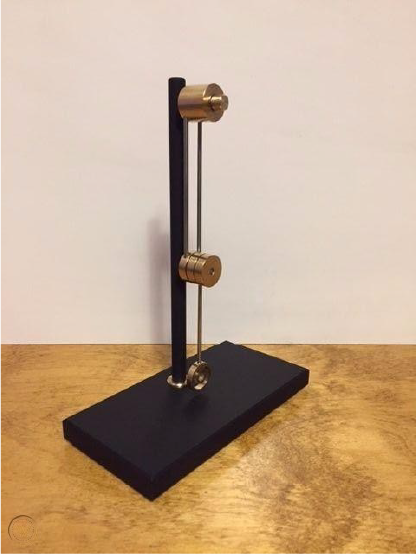
\includegraphics[width=0.9\textwidth]{double-pendulum} % first figure 
            \caption{A double pendulum}
            \label{fig:dbpendulum}
        \end{minipage}\hfill
        \begin{minipage}{0.45\textwidth}
            \centering
            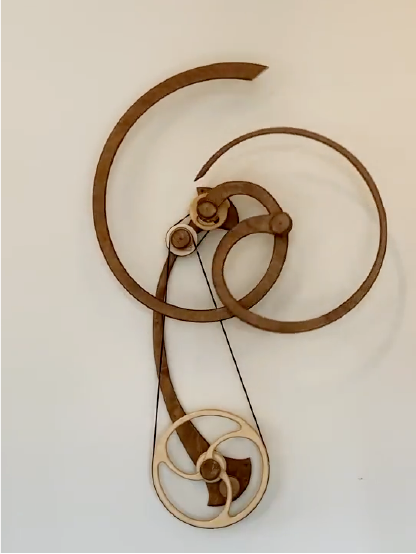
\includegraphics[width=0.9\textwidth]{calli} % second figure
            \caption{Calligraphy}
            \label{fig:calli}
        \end{minipage}
    \end{figure}

    It is the \textbf{aim of this essay} to explore two approaches to analyzing the behavior of the sculpture \textit{“Calligraphy”} (Figure \ref{fig:calli}). The first approach is to find the equations of motion for a simple double pendulum, then use those equations to explore some characteristics of this interesting system, and finally, draw parallels between the simple double pendulum and the sculpture \textit{“Calligraphy”}. The second approach is to produce a probability distribution of the sculpture’s position during a certain span of time. 
    
    This analysis is done to answer the 
    research question: \textit{What is the most probable position of David C. Roy’s kinetic sculpture \textit{“Calligraphy”} would a viewer see if they walk in the exhibition during the first 250 seconds after the sculpture starts running?}

%Definitions
\section{Definitions}
    \begin{enumerate}
        \item \textbf{Pendulum}: A system consisting of a weight suspended from a pivot through a cord/thread/stick that moves back and forth under the effect of gravity. \cite{pendulum}
        \item \textbf{Double pendulum}: A system consisting of one pendulum hanging from the end of another. \cite{double-pendulum}
        \item \textbf{Lagrangian mechanics}: An alternative formulation to Newtonian mechanics, using energies instead of forces to describe motions and dynamics. \cite{lib-lagrangian}
        \item \textbf{Action (physics)}: a functional that describe the overall motion of a physical system \cite{action}. The action is an important quantity because it is used in the stationary action principle, which yields the equations of motion.
        \item \textbf{The stationary action principle}: A principle in mechanical physics, which states that the equations of motion of a system outputs stationary values of the action. \cite{mann-2018}
        \item \textbf{Chaos}: A system is said to be chaotic, or to exhibit chaos when its future state is highly sensitive to its initial conditions, i.e., a small change in initial conditions results in a disproportionately large change in future states. \cite{helsinki}
        \item \textbf{\textit{“Calligraphy”}}: From this point onwards, this term refers to the kinetic sculpture made by artist David C. Roy \cite{roy-2021}. Figure \ref{fig:movement} describes the movement of the sculpture.
    \end{enumerate}
    (Reference to these definitions in the essay will be formatted as: “Definition” in italic + the order number, e.g. \textit{Definition 1})
    \begin{figure}[H]
        \centering
        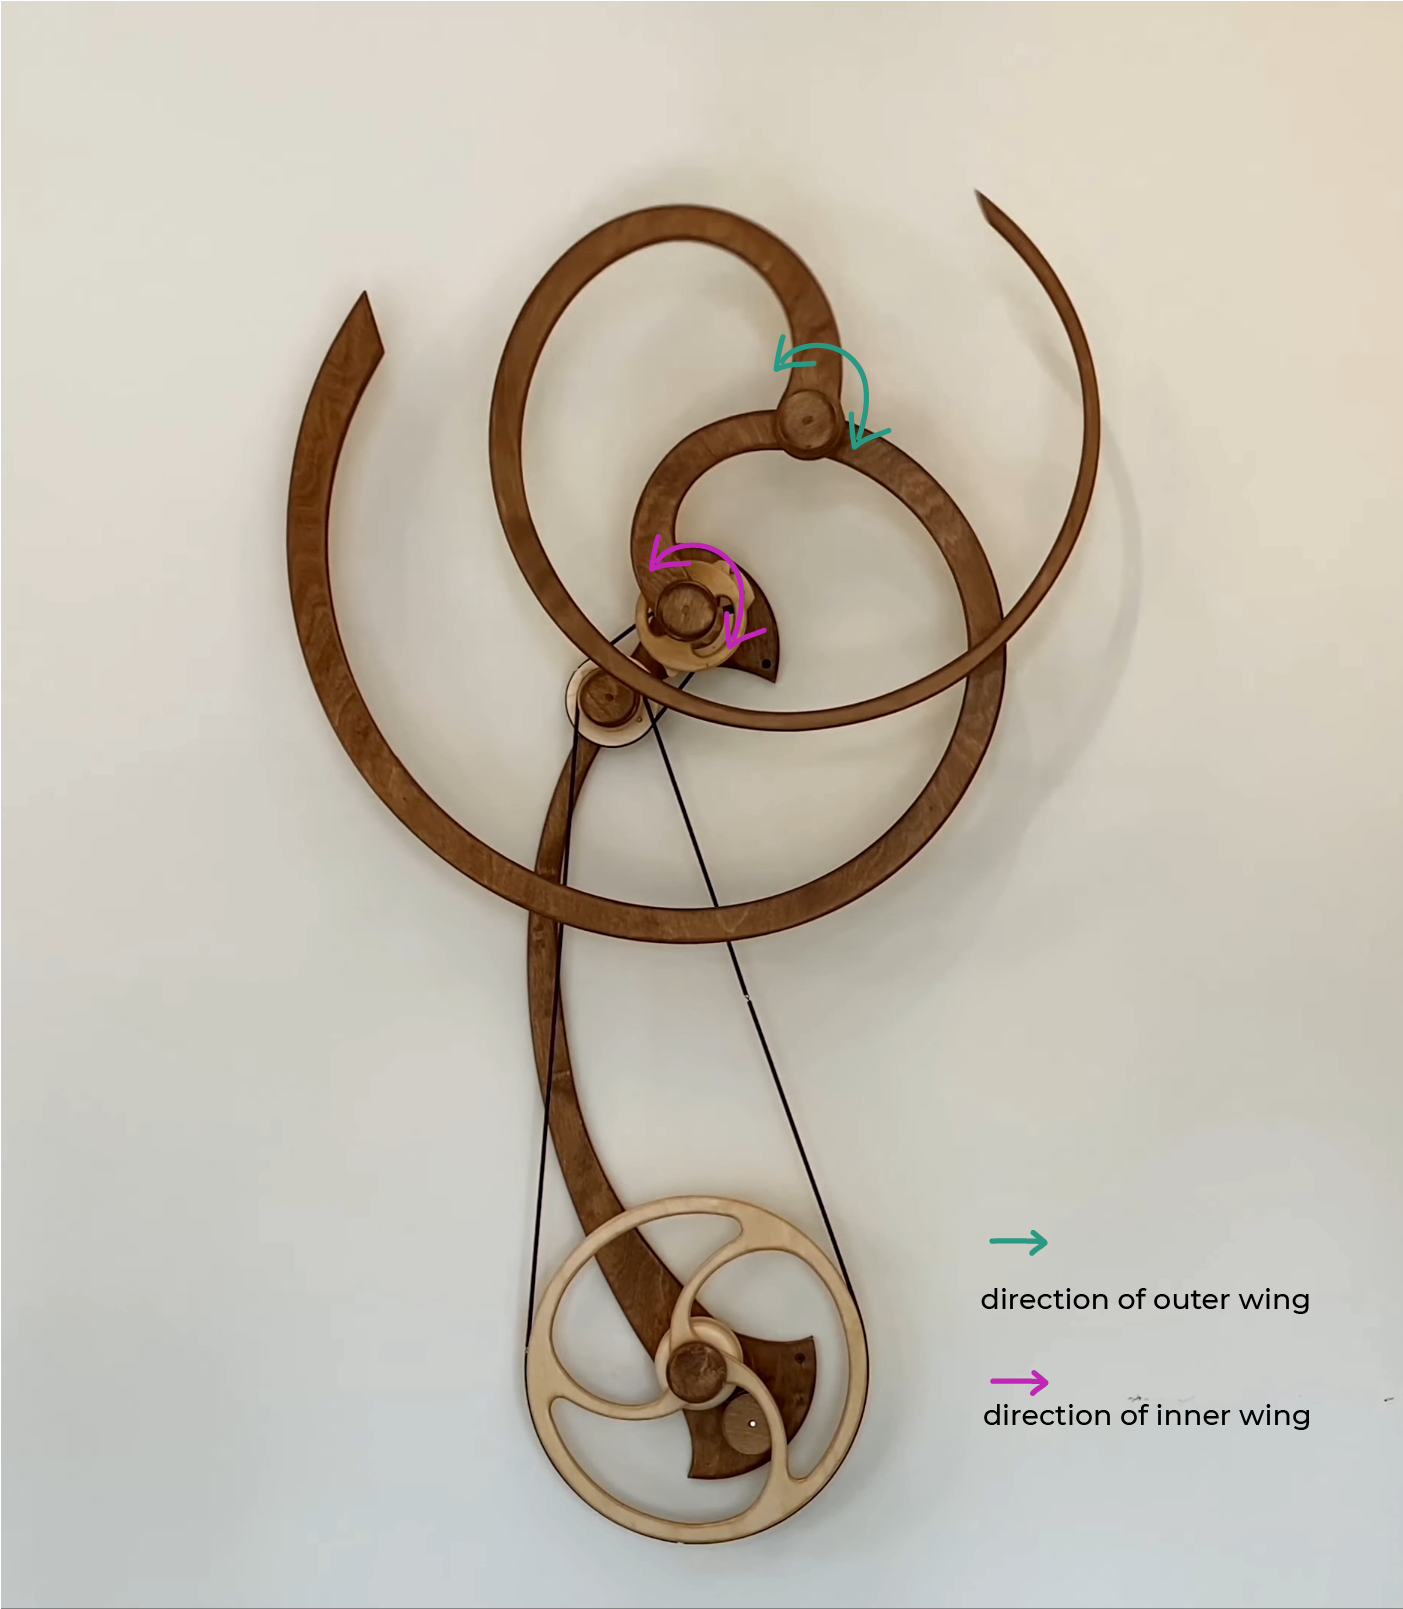
\includegraphics[width=0.5\textwidth]{movement} 
        \caption{Movement of \textit{“Calligraphy”}. Description: The two wings move freely in both direction around its pivot points. The sculpture starts by an external force (e.g. a person pushing), which moves either or both of the wings up, then let it fall down under the effect of gravity. According to the artist \cite{roy-2021}, the two wings would continue moving back and forth for approximately 3 hours.}
        \label{fig:movement}
    \end{figure}

%Approach 1
\section{Approach 1: The simple double pendulum}
To begin with, this essay is going to consider a simple double pendulum - an idealized model consisted of two point-masses attaching at the end of two massless cords (Figure \ref{fig:simpledbp}). In this model, it is assumed there is no friction and air resistance involved.

The general steps to use Lagrangian mechanics to derive the equations of motion for a system is \cite{hirvonen-2022}:
\begin{enumerate}
    \item Find a set of generalized coordinates.
    In this case, it is common to use spherical coordinates ($\theta_1, \theta_2$) to describe the angles that the pendula are displaced from the equilibrium point (where both pendula hang perpendicular to the ground).
    This freedom to pick a convenient set of coordinates is one of the reasons why Lagrangian mechanics is used to solve for the equations of motion in this case. Instead of having to include the effect of constraint forces (the cords constraining the movement to within a circle around the pivot point), one can just use spherical coordinates.
    \pagebreak
    \item Define the Lagrangian through the generalized coordinates (details will be discussed later).
    \item  Substitute the specific Lagrangian to the Euler-Lagrange equation. (details will be discussed later)
    \item Simplify to obtain the equations of motion.
\end{enumerate}

These steps will be further detailed as they are gone through below.
%Step 1 -----------------------------------------------------
\subsection{Find a set of generalized coordinates}
\raggedright{First, the simple double pendulum can be graphed on a two-dimensional Cartesian coordinate system.}
\begin{figure}[H]
    \begin{center}
        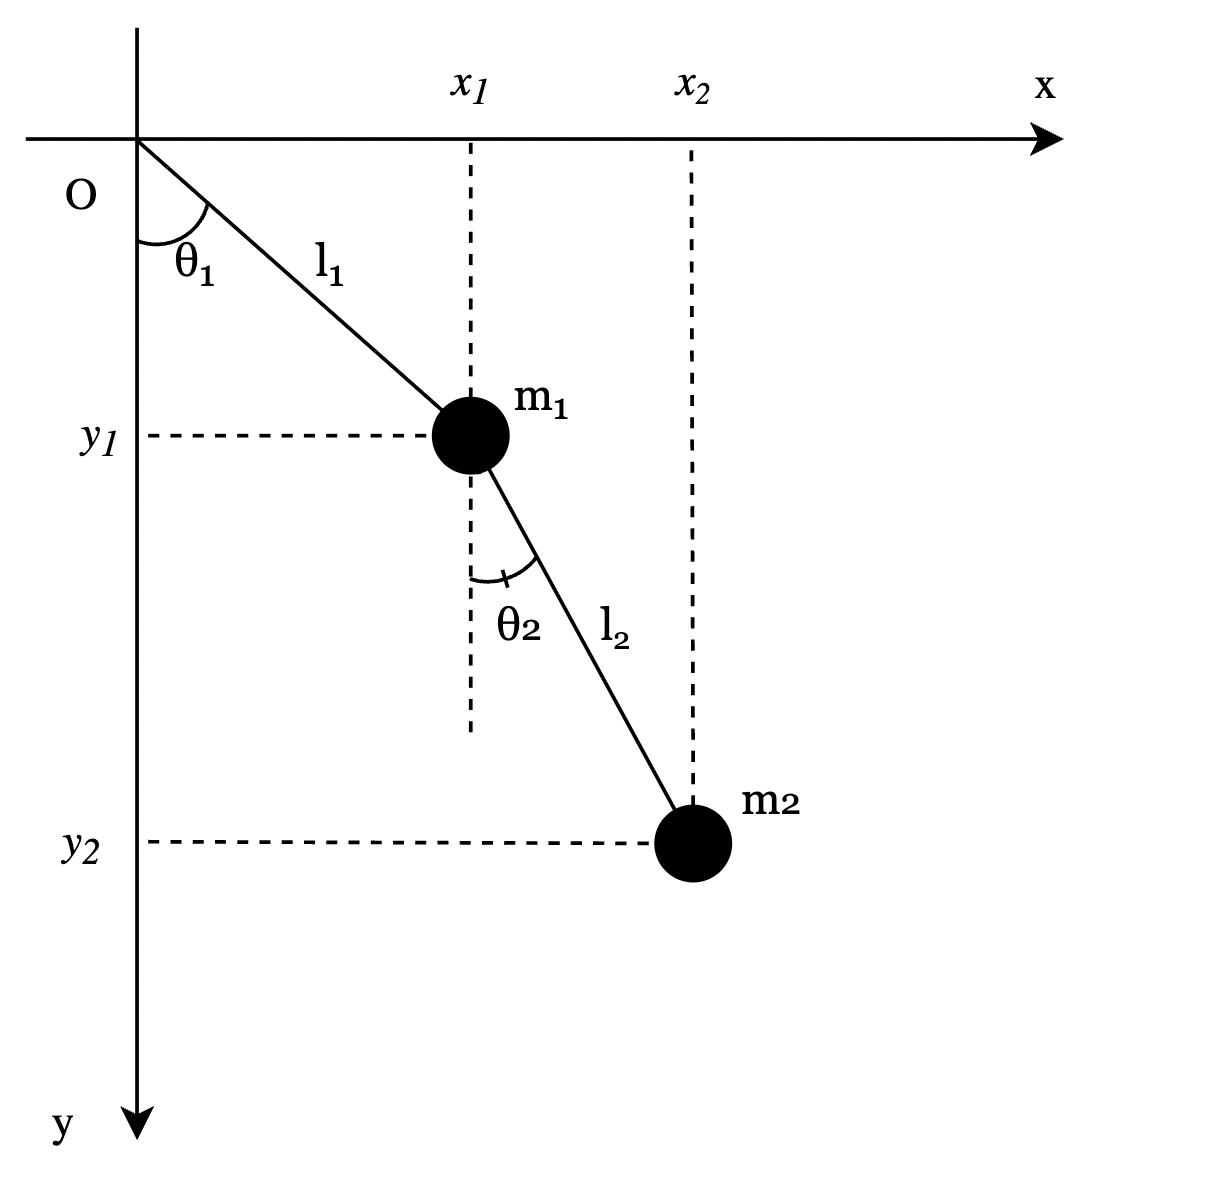
\includegraphics[width=.45\textwidth]{simpledbp} 
    \end{center}
    \caption{}
    \label{fig:simpledbp}
  \end{figure}

In Figure \ref{fig:simpledbp}, the first pendulum consists of a bob with mass $m_1$ suspended at the end of a 
cord with length $l_1$, from the pivot $O(0, 0)$. The second pendulum consists of mass $m_2$ and a cord of length $l_2$, taking the first bob as the pivot point. The angles that the cord of each pendulum makes with the vertical line are respectively $\theta_1$ and $\theta_2$.

\pagebreak The coordinates of the position of each bob is $(x_1,y_1)$ and $(x_2,y_2)$, which can be written in terms of $\theta_1$ and $\theta_2$:

\begin{center}
    $x_1 = l_1sin\theta_1$ 
    
    $y_1=l_1cos\theta_1$
   
    $x_2 = l_1sin\theta_1 \thinspace+\thinspace l_2sin\theta_2$ 
    
    $y_2=l_1cos\theta_1 \thinspace +\thinspace l_2cos\theta_2$ 
\end{center}

We can obtain the instantaneous velocity of each bob by differentiating its position with respect to time. Newton's notation is used to denote the time derivatives ($\dv{f}{t} = \dot{f}$). 
\begin{center}
    $\dot{x_1} = l_1\dot{\theta_1}cos\theta_1$ 
    
    $\dot{y_1}=-l_1\dot{\theta_1}sin\theta_1$
   
    $\dot{x_2} = l_1\dot{\theta_1}cos\theta_1 \thinspace+\thinspace l_2\dot{\theta_2}cos\theta_2$ 
    
    $\dot{y_2}=-l_1\dot{\theta_1}sin\theta_1 \thinspace -\thinspace l_2\dot{\theta_2}sin\theta_2$ 
\end{center}
%Step 2 -----------------------------------------------------
\subsection{Define the Lagrangian}
The Lagrangian is a function that describe the state of a physical system. In classical
mechanics, it is defined as the difference between kinetic and potential energy \cite{lagrangian-func}.

In this system containing two objects, the Lagrangian is the sum of the difference between kinetic and potential energy of each object:
\begin{center}\[L=\sum_{i=1}^{2 }T_i-\sum_{i=1}^{2 }V_i\]\end{center}
where:
\begin{conditions}
    L & the Lagrangian \\
    m & mass \\
    v & velocity \\
    T & kinetic energy \\
    V & potential energy \\ 
    i & index number of the object (our system has two objects, thus i runs from 1 to 2)
\end{conditions} 
The expressions for the instantaneous velocities found in subsection 3.1 are substituted in this equation. That gives an expression for the kinetic energy $T$ in terms of $\theta_1$ and $\theta_2$ as: 
\begin{align*}
    \begin{split}
        T &= \frac{1}{2}\sum_{i=1}^{ 2}m_iv_i^2 
    \end{split}\\
    \begin{split}
        &= \frac{1}{2}  m_1(\dot{x_1}^2+\dot{y_1}^2)\thinspace + \thinspace \frac{1}{2}m_2(\dot{x_2}^2+\dot{y_2}^2)
    \end{split}\\
        %\begin{multline}
            &=\frac{1}{2}m_1[(l_1)^2\dot{\theta_1}^2cos^2\theta_1 + (l_1)^2 \dot{\theta_1}^2sin^2\theta_1] \thinspace + \thinspace \frac{1}{2}m_2[ (l_1)^2\dot{\theta_1}^2cos^2\theta_1 +2l_1l_2\dot{\theta_1}\dot{\theta_2}cos\theta_1cos\theta_2
            \\&\space +(l_2)^2\dot{\theta_2}^2cos^2\theta_2 \thinspace + \thinspace (l_1)^2\dot{\theta_1}^2sin^2\theta_1 +2l_1l_2\dot{\theta_1}\dot{\theta_2}sin\theta_1sin\theta_2+(l_2)^2\dot{\theta_2}^2sin^2\theta_2] 
        %\end{multline}
\end{align*}

Since $cos^2x+sin^2x=1$ for all $x$:
\[T =\frac{1}{2}m_1(l_1)^2\dot{\theta_1}^2
+\frac{1}{2}m_2(l_1)^2\dot{\theta_1}^2+\frac{1}{2}m_2.[2l_1l_2\dot{\theta_1}\dot{\theta_2}(cos\theta_1cos\theta_2+sin\theta_1sin\theta_2)]+\frac{1}{2}m_2(l_2)^2\dot{\theta_2}^2\]

We have $cos\theta_1cos\theta_2+sin\theta_1sin\theta_2=cos(\theta_1-\theta_2)$, thus the equation becomes:
\begin{equation}
    T=\frac{1}{2}(m_1+m_2)(l_1)^2\dot{\theta_1}^2+\frac{1}{2}m_2[2l_1l_2\dot{\theta_1}\dot{\theta_2}cos(\theta_1-\theta_2)+(l_2)^2\dot{\theta_2}^2]
\end{equation}

Likewise, the potential energy can be expressed in terms of $\theta_1$ and $\theta_2$. In the graph, the height of the bob is $-y_i$, since the y-axis points downwards. So the potential energy $V$ can be expressed as:
\begin{align*}
    V &= \sum_{i=1}^{2 }m_ig(-y_i)
    \\&= m_1g(-y_1) +m_2g(-y_2)
    \\&= -g(m_1l_1cos\theta_1 +m_2l_1cos\theta_1+m_2l_2cos\theta_2)
\end{align*}
Expanded and rearranged as:
\begin{equation}
    V   = -g(m_1+m_2)l_1cos\theta_1 \space - \space gm_2l_2cos\theta_2
\end{equation}

The classical Lagrangian is defined above as $L = T-V$. Substituting $(1)$ and $(2)$ into this equation, we have:
\begin{multline}
    L=\frac{1}{2}(m_1+m_2)(l_1)^2\dot{\theta_1}^2+\frac{1}{2}m_2[2l_1l_2\dot{\theta_1}\dot{\theta_2}cos(\theta_1-\theta_2)+(l_2)^2\dot{\theta_2}^2] \\
    +g(m_1+m_2)l_1cos\theta_1 \space + \space gm_2l_2cos\theta_2 
\end{multline}
%Step 3 -----------------------------------------------------
\subsection{Apply the Euler-Lagrange equations and simplify}
In order to implement this step, partial derivatives are needed. Similar to ordinary derivatives, they describe the rate of change of an output of a function with respect to one of its input. However, unlike ordinary derivative where the function has only one variable, partial derivative is “partial” since the function has multiple variables, and the derivative is taken with respect to only one of them. The website WorldFram MathWorld defines partial derivatives as “derivatives of a function of multiple variables when all but the variable of interest are held fixed during the differentiation” \cite{partial-derivative}. The notation for a partial derivative of function $f(x,y)$ with respect to $x$ is $\frac{\partial f(x,y)}{\partial x}$.

The Euler-Lagrange equation is a result from calculus of variations \cite{fox-2010}. In Lagrangian mechanics, this equation ensures the system satisfy the principle of stationary action (\textit{Definition 5}). For each generalized coordinate $q_i$, the Euler-Lagrange equation is given as:
\[
\dv{}{t}\frac{\partial L}{\partial \dot{q_i}}=\frac{\partial L}{\partial q_i}, i = 1,...,n
\]
where:
\begin{conditions}
    L & the Lagrangian function\\
    n & number of coordinates in the system\\
    t & time
\end{conditions}
It is helpful to note that while $\dot{q}$ is the derivative with respect to time of $q$, here they are treated as two separate variables.

Now that the Lagrangian for the simple double pendulum has been defined in equation $(3)$, the Euler-Lagrange equation can be applied to find the equations of motion. 

For $\theta_1$:
\begin{equation}
    \dv{}{t}\frac{\partial L}{\partial \dot{\theta_1}}=\frac{\partial L}{\partial \theta_1}
    \end{equation}

Substitute $(3)$ for L, the left side of equation $(4)$ expands as:
\begin{align*}
    &\dv{}{t}\frac{\partial}{\partial \dot \theta_1}
    \{\frac{1}{2}(m_1+m_2)l_1^2\dot{\theta_1}^2+\frac{1}{2}m_2[2l_1l_2\dot{\theta_1}\dot{\theta_2}cos(\theta_1-\theta_2)]\}
    \\
    ={} &\dv{}{t}[(m_1+m_2)l_1^2\dot \theta_1+m_2l_1l_2\dot \theta_2cos(\theta_1-\theta_2)]
    \\
    ={} &(m_1+m_2)l_1^2\ddot\theta_1+m_2l_1l_2[\ddot \theta_2cos(\theta_1-\theta_2) - \dot\theta_2sin(\theta_1-\theta_2)(\dot \theta_1 - \dot \theta_2)]
\end{align*}
\begin{multline}
    =(m_1+m_2)l_1^2\ddot\theta_1+m_2l_1l_2\ddot\theta_2cos(\theta_1-\theta_2)-m_2l_1l_2\dot\theta_1\dot\theta_2sin(\theta_1-\theta_2)\\
    +m_2l_1l_2\dot\theta_2^2sin(\theta_1-\theta_2)
\end{multline}
And the right side of $(4)$:
\begin{align*}
    &\frac{\partial}{\partial \theta_1}
    \{\frac{1}{2}m_2[2l_1l_2\dot{\theta_1}\dot{\theta_2}cos(\theta_1-\theta_2)]
    +g(m_1+m_2)l_1cos\theta_1\}
    \\
    ={}&\frac{\partial}{\partial \theta_1}
    [m_2l_1l_2\dot{\theta_1}\dot{\theta_2}(cos\theta_1\theta_2+sin\theta_1sin\theta_2)
    +g(m_1+m_2)l_1cos\theta_1]
    \\
    ={}&m_2l_1l_2\dot{\theta_1}\dot{\theta_2}(-sin\theta_1\theta_2+cos\theta_1sin\theta_2)
    -g(m_1+m_2)l_1sin\theta_1
\end{align*}
%Right side theta 1
\begin{equation}
    = -m_2l_1l_2\dot\theta_1 \dot\theta_2sin(\theta_1-\theta_2) -g(m_1+m_2)l_1sin\theta_1
\end{equation}

Substituting $(5)$ and $(6)$ into the left and right side of $(4)$:
\begin{multline*}
    (m_1+m_2)l_1^2\ddot\theta_1+m_2l_1l_2\ddot\theta_2cos(\theta_1-\theta_2)-m_2l_1l_2\dot\theta_1\dot\theta_2sin(\theta_1-\theta_2)+m_2l_1l_2\dot\theta_2^2sin(\theta_1-\theta_2)
    \\=-m_2l_1l_2\dot\theta_1 \dot\theta_2sin(\theta_1-\theta_2)
    -g(m_1+m_2)l_1sin\theta_1
\end{multline*}
\[
    \therefore(m_1+m_2)l_1^2\ddot\theta_1+m_2l_1l_2[\ddot\theta_2cos(\theta_1-\theta_2)+\dot\theta_2^2sin(\theta_1-\theta_2)]+g(m_1+m_2)l_1sin\theta_1=0
\]

Cancelling $l_1$ and rearranging:
\begin{equation}
    (m_1+m_2)(l_1\ddot\theta_1+gsin\theta_1)+m_2l_2[\ddot\theta_2cos(\theta_1-\theta_2)+\dot\theta_2^2sin(\theta_1-\theta_2)] =0
\end{equation}

Similarly, for $\theta_2$:
\begin{equation}\dv{}{t}\frac{\partial L}{\partial \dot{\theta_2}}=\frac{\partial L}{\partial \theta_2}\end{equation}
Left side: 
\begin{align*}
    &\frac{d}{dt}\frac{\partial}{\partial \dot{\theta_2}}[\frac{1}{2}m_2l_2^2\dot\theta_2^2+m_2l_1l_2\dot\theta_1\dot\theta_2cos(\theta_1-\theta_2)]
    \\
    ={}&\frac{d}{dt}[m_2l_2^2\dot\theta_2+m_2l_1l_2\dot\theta_1cos(\theta_1-\theta_2)]
    \\
    ={}&m_2l_2^2\ddot\theta_2+m_2l_1l_2[\ddot\theta_1cos(\theta_1-\theta_2)-\dot\theta_1sin(\theta_1-\theta_2)(\dot\theta_1-\dot\theta_2)]
\end{align*}
\begin{equation}
    =m_2l_2^2\ddot\theta_2+m_2l_1l_2\ddot\theta_1cos(\theta_1-\theta_2)-m_2l_1l_2\dot\theta_1^2sin(\theta_1-\theta_2)+m_2l_1l_2\dot\theta_1\dot\theta_2sin(\theta_1-\theta_2)
\end{equation}

Right side:
\begin{align*}
    &\frac{\partial}{\partial \theta_2}[m_2l_1l_2\dot\theta_1\dot\theta_2cos(\theta_1-\theta_2)+gm_2l_2cos\theta_2]
    \\
    ={}&\frac{\partial}{\partial \theta_2}[m_2l_1l_2\dot\theta_1\dot\theta_2(cos\theta_1 cos\theta_2+sin\theta_1 sin\theta_2)+gm_2l_2cos\theta_2]
    \\
    ={}&m_2l_1l_2\dot\theta_1\dot\theta_2(-cos\theta_1 sin\theta_2+sin\theta_1 cos\theta_2)-gm_2l_2sin\theta_2
\end{align*}
\begin{equation}
    =m_2l_1l_2\dot\theta_1\dot\theta_2sin(\theta_1-\theta_2)-gm_2l_2sin\theta_2
\end{equation}

Substituting $(9)$ and $(10)$ into $(8)$, we obtain the second equation of motion:
\begin{multline*}
m_2l_2^2\ddot\theta_2+m_2l_1l_2\ddot\theta_1cos(\theta_1-\theta_2)-m_2l_1l_2\dot\theta_1^2sin(\theta_1-\theta_2)+m_2l_1l_2\dot\theta_1\dot\theta_2sin(\theta_1-\theta_2)
\\
= m_2l_1l_2\dot\theta_1\dot\theta_2sin(\theta_1-\theta_2)-gm_2l_2sin\theta_2
\end{multline*}
\[\therefore m_2l_2^2\ddot\theta_2+m_2l_1l_2\ddot\theta_1cos(\theta_1-\theta_2)-m_2l_1l_2\dot\theta_1^2sin(\theta_1-\theta_2)+gm_2l_2sin\theta_2=0\]

Cancelling $m_2l_2$:
\begin{equation}
    l_2\ddot\theta_2+l_1\ddot\theta_1cos(\theta_1-\theta_2)-l_1\dot\theta_1^2sin(\theta_1-\theta_2)+gsin\theta_2=0
\end{equation}
Equations $(7)$ and $(11)$ form the system of equations of motion that describe the behavior of the simple double pendulum over time. They form a highly non-linear system of two second-order differential equations, hinting at the complexity of the behavior of the system:
\begin{equation*}
    \begin{cases}
        (m_1+m_2)(l_1\ddot\theta_1+gsin\theta_1)+m_2l_2[\ddot\theta_2cos(\theta_1-\theta_2)+\dot\theta_2^2sin(\theta_1-\theta_2)] =0 
    \\
        l_2\ddot\theta_2+l_1\ddot\theta_1cos(\theta_1-\theta_2)-l_1\dot\theta_1^2sin(\theta_1-\theta_2)+gsin\theta_2=0
    \end{cases}
\end{equation*} 
%Step 4 -----------------------------------------------------
\subsection{Plot generation}
These equation can be solved using the differential equation solver ode113 in the software MATLAB. To clean up the code for readability, we can rearrange the terms by putting all terms not containing $\ddot{\theta_1}$ and $\ddot{\theta_2}$ to the right, then divide both sides of (7) by the coefficients of $\ddot{\theta_1}$ and (11) by the coefficients of $\ddot{\theta_2}$.

So, equation (7) can be written as:
\begin{align*}
    \ddot\theta_1  + \ddot\theta_2\frac{m_2}{m_1+m_2}\frac{l_2}{l_1}cos(\theta_1-\theta_2)=  -\frac{g}{l_1}sin\theta_1 -\frac{m_2}{m_1+m_2}\frac{l_2}{l_1}\dot\theta_2^2sin(\theta_1-\theta_2)
\end{align*}
Equation (11) can be written as:
\begin{align*}
    \ddot\theta_2 + \ddot\theta_1\frac{l_1}{l_2}cos(\theta_1-\theta_2)=\frac{l_1}{l_2}\dot\theta_1^2sin(\theta_1-\theta_2) - \frac{g}{l_2}sin\theta_2
\end{align*}

These equations can be respectively represented as:
\begin{equation}
    \ddot\theta_1  + \ddot\theta_2\alpha_1=f_1
\end{equation}
\begin{equation}
    \ddot\theta_2  + \ddot\theta_1\alpha_2=f_2
\end{equation}
where:
\begin{equation}
    \alpha_1 = \frac{m_2}{m_1+m_2}\frac{l_2}{l_1}cos(\theta_1-\theta_2)
\end{equation}
\begin{equation}
    \alpha_2 = \frac{l_1}{l_2}cos(\theta_1-\theta_2)
\end{equation}
\begin{equation}
    f_1= -\frac{g}{l_1}sin\theta_1 -\frac{m_2}{m_1+m_2}\frac{l_2}{l_1}\dot\theta_2^2sin(\theta_1-\theta_2)
\end{equation}
\begin{equation}
    f_2=\frac{l_1}{l_2}\dot\theta_1^2sin(\theta_1-\theta_2) - \frac{g}{l_2}sin\theta_2
\end{equation}

Equations (12) and (13) can now be entered into MATLAB (see Appendix A for the source code). A simple double pendulum with lengths and masses all equal 1 is considered.

For small angle release of $\theta_1 = \pi/12$ and $\theta_2=0$, periodic movement is observed (Figure \ref{fig:pi12}).
\pagebreak

\begin{figure}[H]
    \centering
    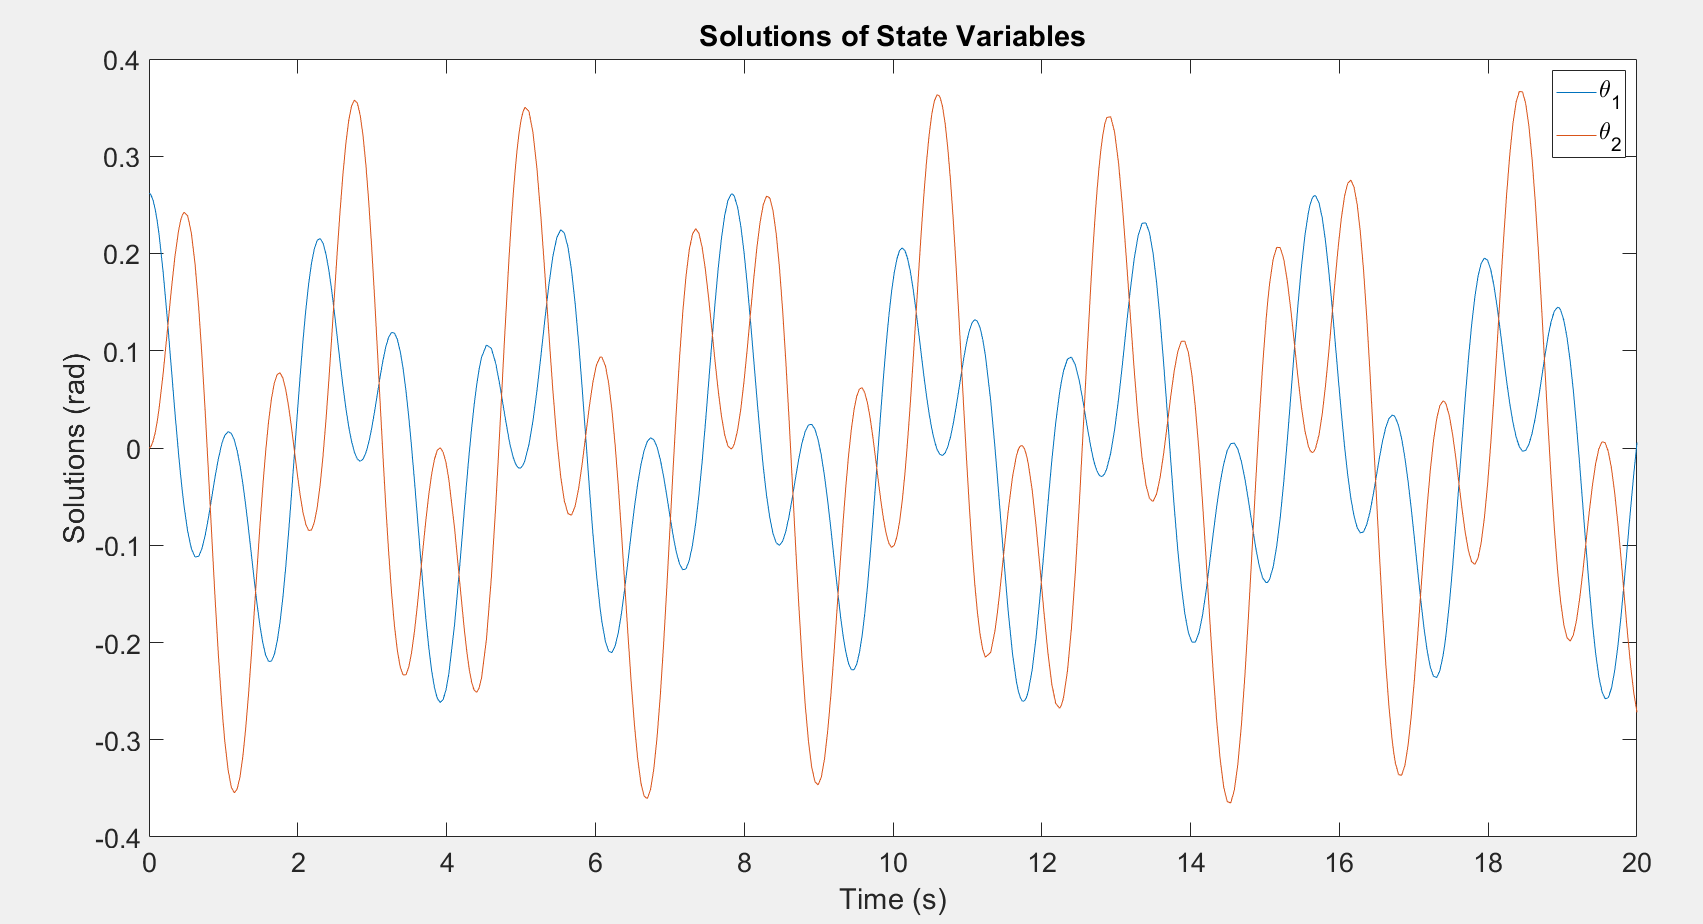
\includegraphics[width=.9\textwidth]{pi12}
    \caption{Graph of $\theta_1$ and $\theta_2$ during first 20 seconds, for $g = 9.8$, $m_1 = m_2 = 1$, $l_1 = l_2 = 1$. Initial angles: $\theta_1 = \pi/12$ and $\theta_2=0$. Command used: ode113. Software used: MATLAB}
    \label{fig:pi12}
\end{figure}

Compare Figure \ref{fig:pi12} to Figure \ref{fig:pi12-001}, when $\theta_1$ is increased by 0.001:
\begin{figure}[H]
    \centering
    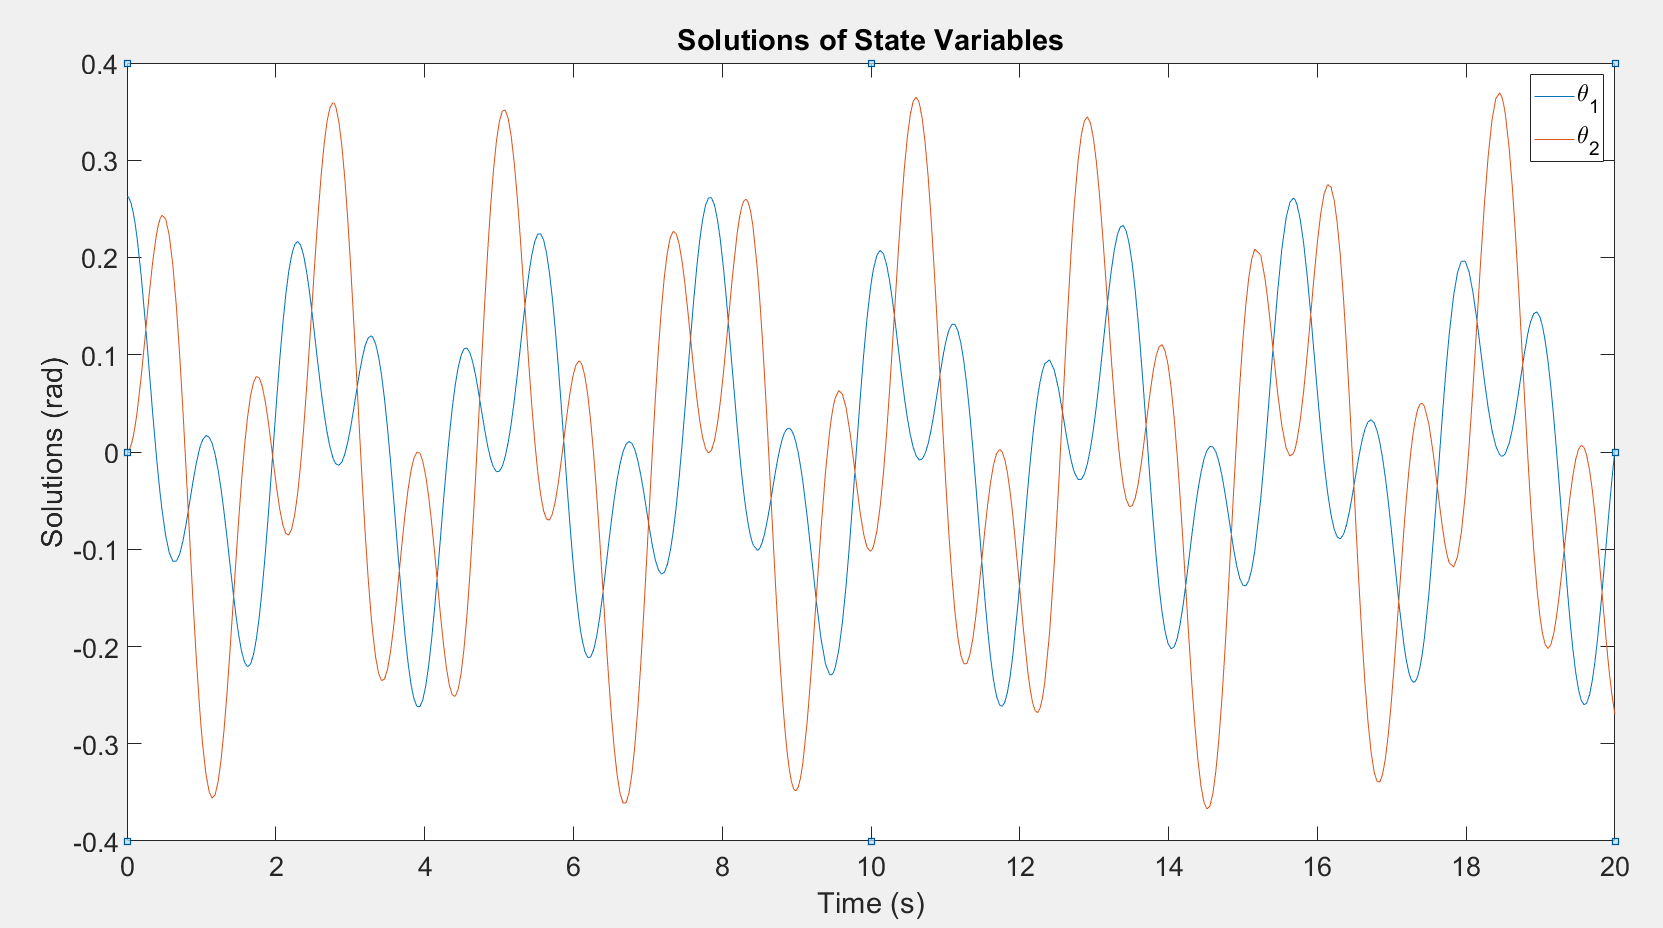
\includegraphics[width=.9\textwidth]{pi12-001}
    \caption{Graph of $\theta_1$ and $\theta_2$ during first 20 seconds, for $g = 9.8$, $m_1 = m_2 = 1$, $l_1 = l_2 = 1$. Initial angles: $\theta_1 = \pi/12+ 0.001$ and $\theta_2=0$. Command used: ode113. Software used: MATLAB}
    \label{fig:pi12-001}
\end{figure}
It can be observed that the very small change in initial conditions (+0.001 rad) results in a proportionately very small change in outputs. 

However, for big angle release, the behavior of $\theta_2$ becomes aperiodic in just 3 seconds:
\begin{figure}[H]
    \centering
    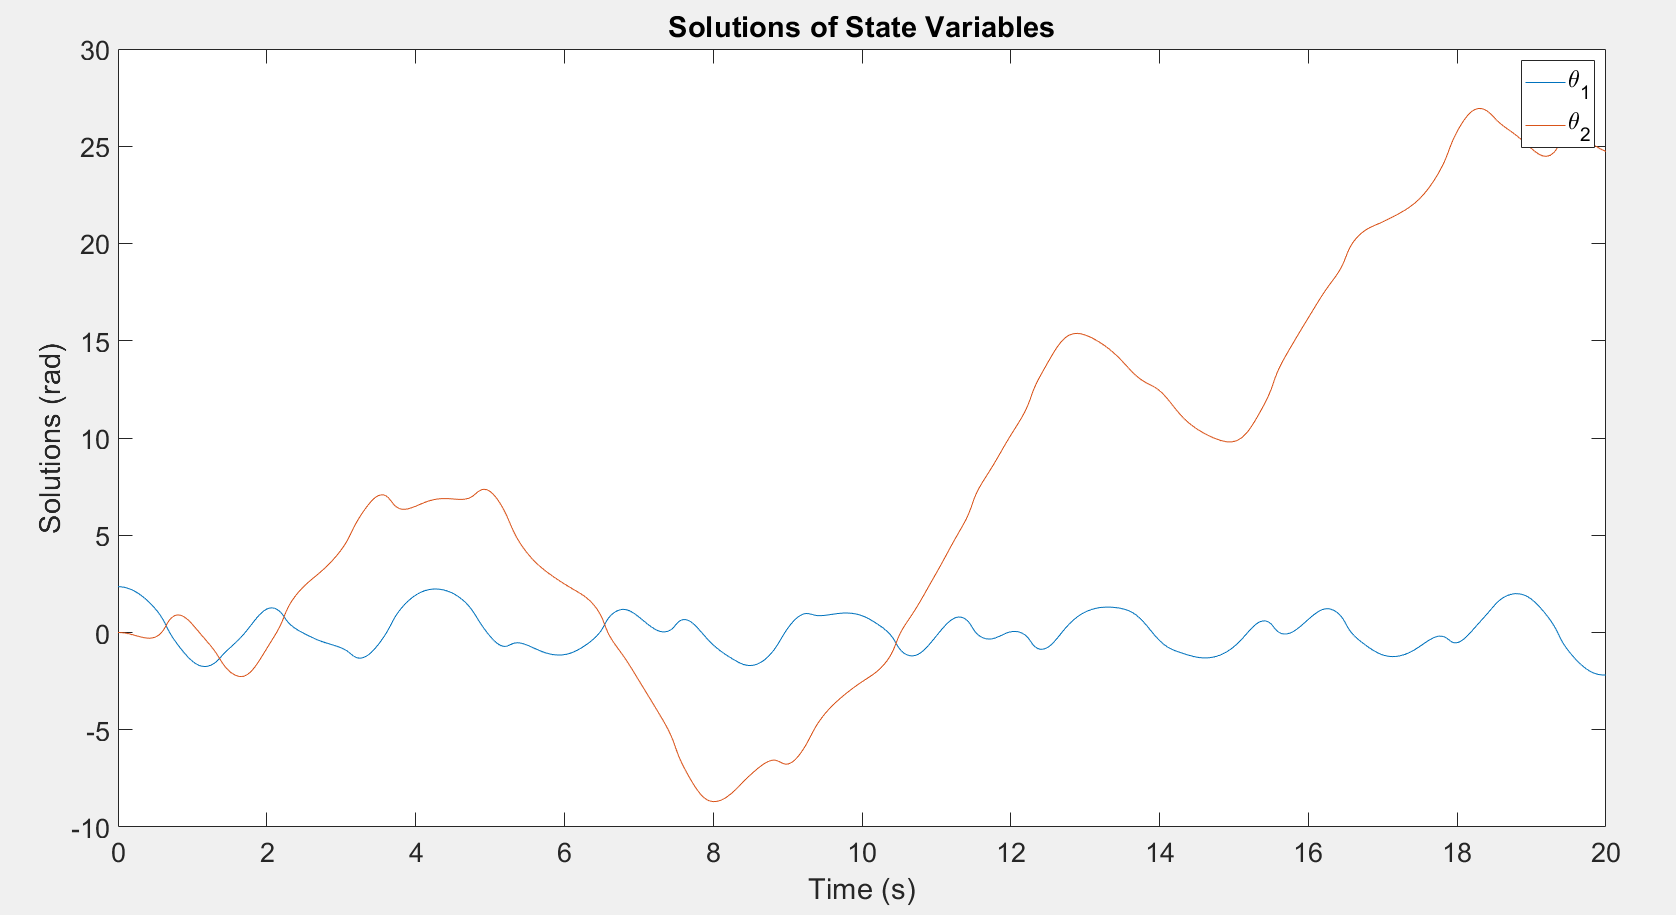
\includegraphics[width=.9\textwidth]{3pi4}
    \caption{Graph of $\theta_1$ and $\theta_2$ during first 20 seconds, for $g = 9.8$, $m_1 = m_2 = 1$, $l_1 = l_2 = 1$. Initial angles: $\theta_1 = 3\pi/4$ and $\theta_2=0$. Command used: ode113. Software used: MATLAB}
    \label{fig:3pi4}
\end{figure}

This time, when initial condition of $\theta_1$ is increased by 0.001, the resulting trajectory of the double pendulum is changed significantly (Figure \ref{fig:3pi4-001}).
\begin{figure}[H]
    \centering
    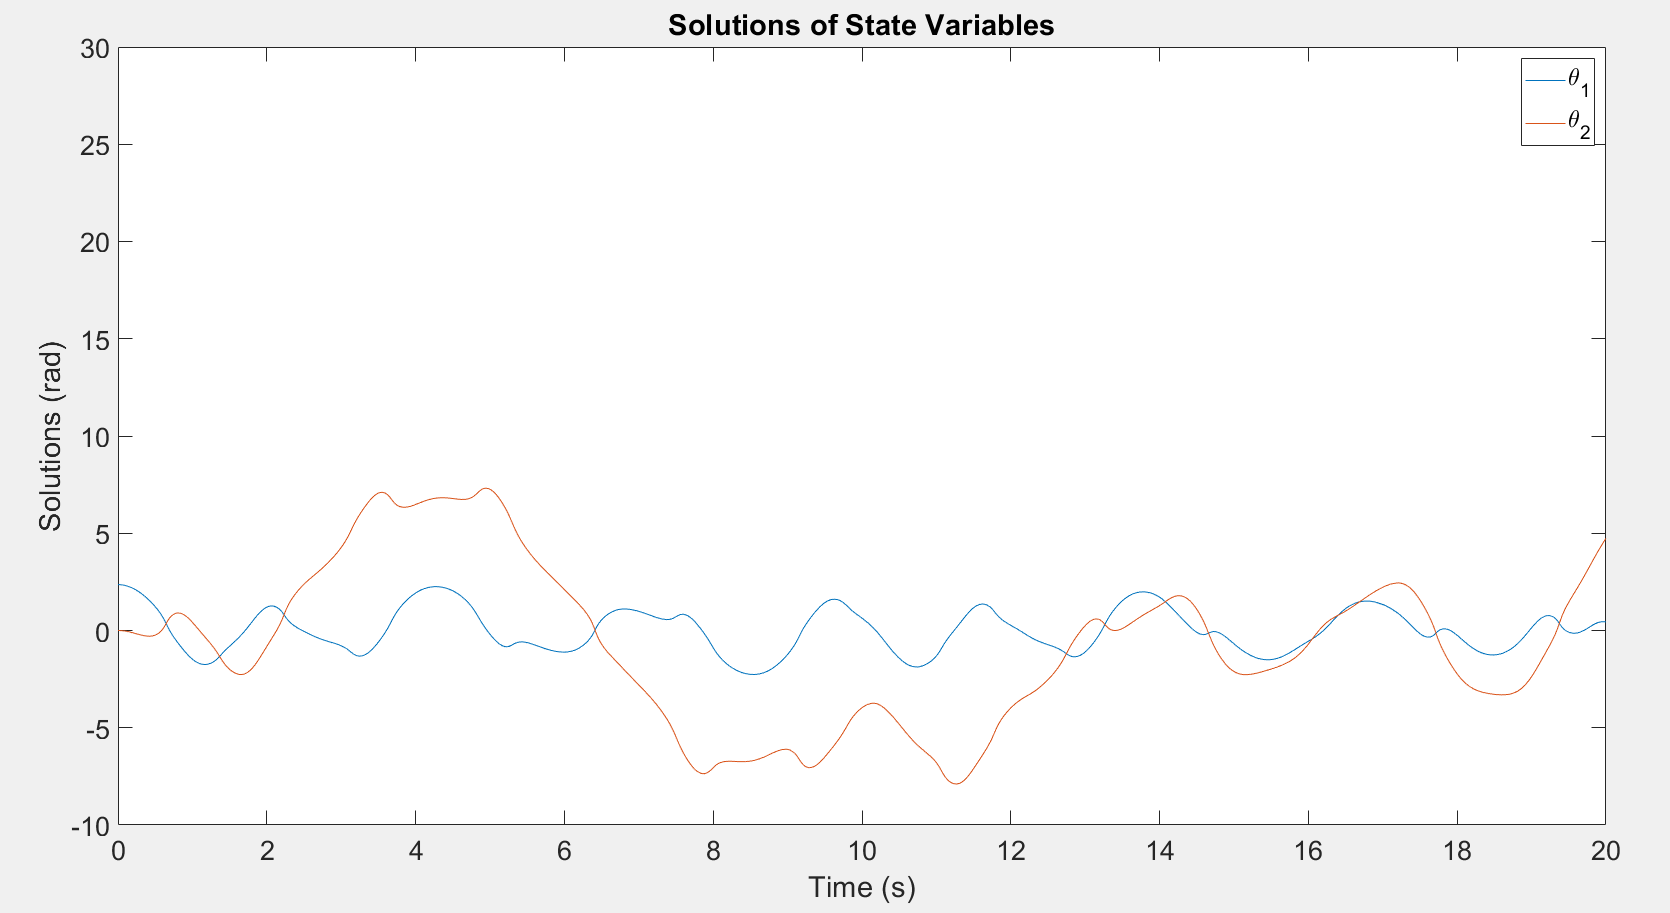
\includegraphics[width=.9\textwidth]{3pi4-001}
    \caption{Graph of $\theta_1$ and $\theta_2$ during first 20 seconds, for $g = 9.8$, $m_1 = m_2 = 1$, $l_1 = l_2 = 1$. Initial angles: $\theta_1 = 3\pi/4+0.001$ and $\theta_2=0$. Command used: ode113. \\Software used: MATLAB}
    \label{fig:3pi4-001}
\end{figure}
This sensitivity to initial conditions is a hallmark of chaos (\textit{Definition 6}). 

These results show that the behavior of the double pendulum can be periodic for small-angle release, but chaotic for large-angle release. 
%Limitations 1st approach -----------------------------------
\subsection{Limitations of the first approach}
These graphs gives a helpful idea about how a simpler but still similar system exhibits behavior of chaos. However, the sculpture \textit{“Calligraphy”} is more complicated than the simple double pendulum in crucial ways.

Comparing Figure \ref{fig:lbdbpendulum} and Figure \ref{fig:lbcalli}, it can be seen that while both systems contains of two pivots and two free swinging masses.
\begin{figure}[H]
    \centering
    \begin{minipage}{0.45\textwidth}
        \centering
        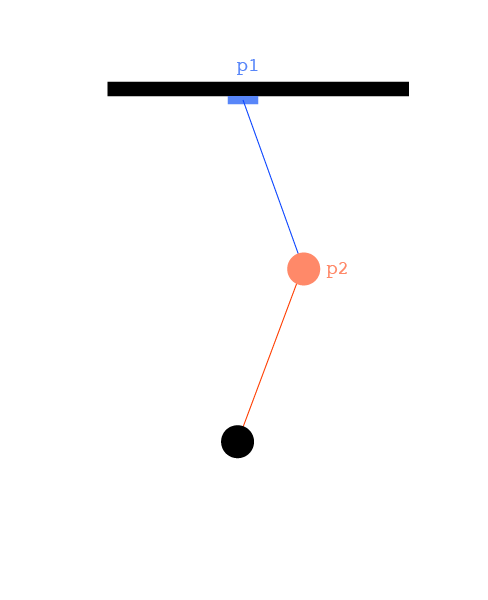
\includegraphics[width=0.9\textwidth]{labelled_double_pendulum} % first figure 
        \caption{Labelled simple double pendulum}
        \label{fig:lbdbpendulum}
    \end{minipage}\hfill
    \begin{minipage}{0.45\textwidth}
        \centering
        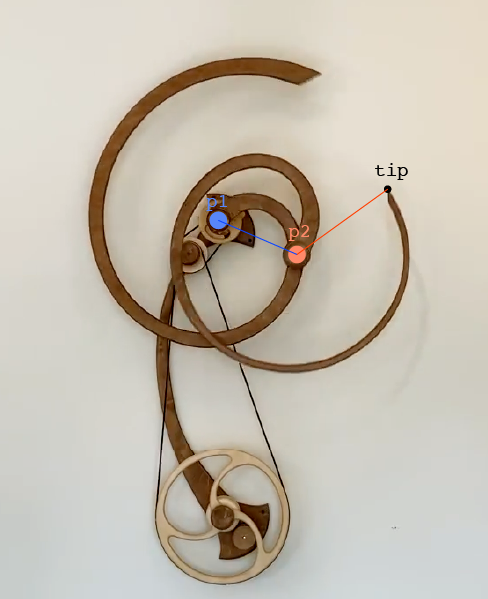
\includegraphics[width=0.9\textwidth]{labelled_sculpt} % second figure
        \caption{Labelled \textit{“Calligraphy”}}
        \label{fig:lbcalli}
    \end{minipage}
\end{figure}

However, the distribution of masses and the forces included is different. In the simple double pendulum, the mass of the first pendulum is entirely concentrated at the end of the massless cords (Figure \ref{fig:mass-db}), and the pivot point of the second pendulum (labelled "p2" in the figure) coincides with that end point. Meanwhile, in the sculpture \textit{“Calligraphy”}, the mass is distributed along the wing (Figure \ref{fig:mass-ca}). This means the pivot point of the second wing is not necessarily at the centre of mass of the first wing.
\begin{figure}[H]
    \centering
    \begin{minipage}{0.45\textwidth}
        \centering
        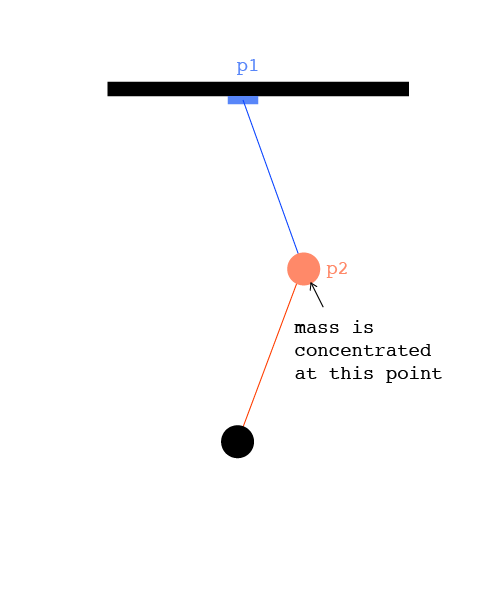
\includegraphics[width=.9\textwidth]{dif_labelled_double_pendulum}
        \caption{}
        \label{fig:mass-db}
    \end{minipage}\hfill
    \begin{minipage}{0.45\textwidth}
        \centering
        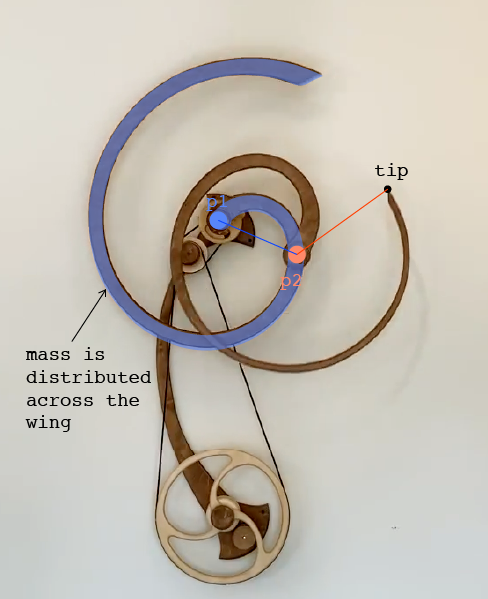
\includegraphics[width=.9\textwidth]{dif_labelled_sculpt}
        \caption{}
        \label{fig:mass-ca}
    \end{minipage}
\end{figure}

Furthermore, there are more forces involved in the system of \textit{“Calligraphy”} compared to the simple double pendulum. The only external forces involved in the system of the simple double pendulum is the initial force and gravity. Meanwhile, the behavior of \textit{“Calligraphy”} also involves force from a spring (Figure \ref{fig:spring}). 
\begin{figure}[H]
    \centering
    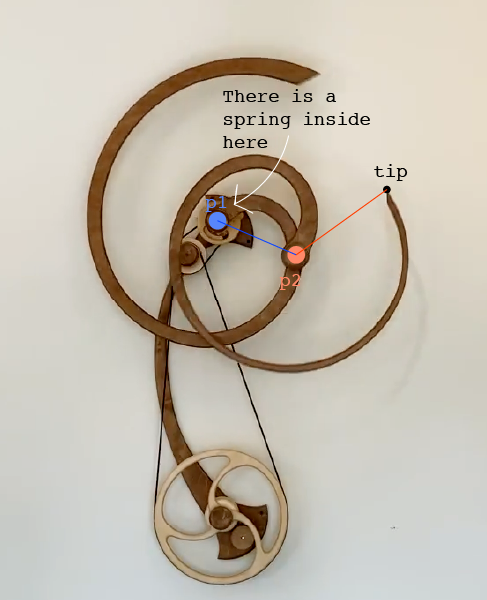
\includegraphics[width=.5\textwidth]{springs}
    \caption{}
    \label{fig:spring}
\end{figure}

Moreover, during operation, \textit{“Calligraphy”} is affected by dissipative forces such as friction, air resistance, in contrast to the idealistic model of the simple double pendulum where it is assumed no such force is present.

This complicates the relationship between the initial angle release and the position of the wings at a particular point of time afterwards. The scope of that is beyond this essay, so it will not try to derive the equations of motions for \textit{“Calligraphy”}. 

Instead, an alternative approach can be employed to study the behaviour of the sculpture. In this approach, the position of the tip (labelled in black in Figure \ref{fig:lbdbpendulum}), is traced over 250 seconds from initial release, in a video of the sculpture \cite{roy-2021}.

%Approach 2   
\section{Approach 2: Probability distribution of tip position}
\subsection{Data collection}

In the software Logger Pro, a video recording of the sculpture \cite{roy-2021} is imported. The data being obtained is the position of the tip of “Calligraphy” over time. Using the “Add point” function of the software, a pair coordinates (X, Y) describing the position of the point is recorded at each frame. There are 7490 points corresponded with 7490 frames recorded over a period of 250 seconds from initial release. This data is then exported to a .csv file, which is then imported to MS Excel to perform analysis on.

\subsection{Data analysis}

\begin{figure}[H]
    \begin{center}
        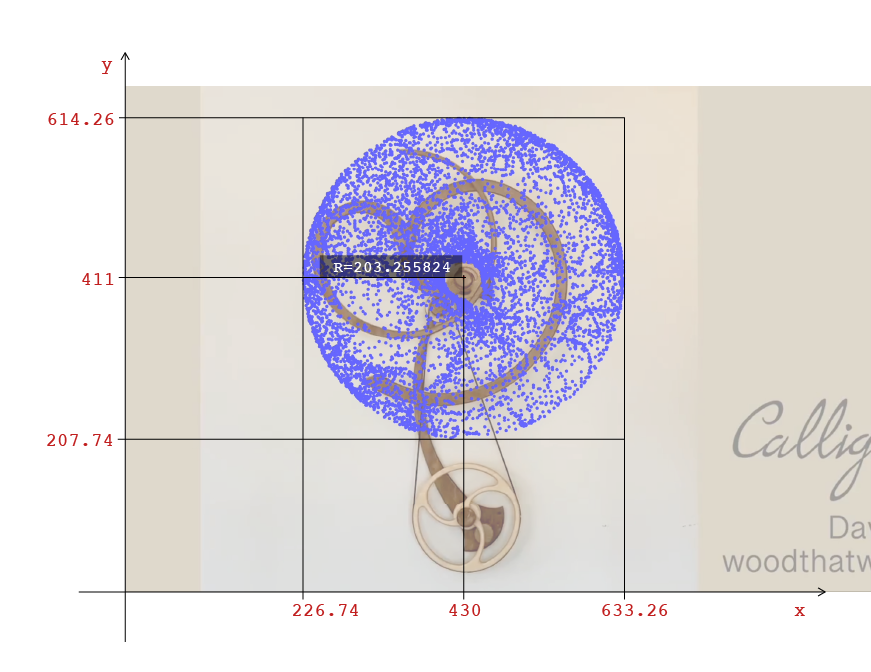
\includegraphics[width=\textwidth]{sculpt-cartesian} 
    \end{center}
    \caption{Coordinate system on the sculpture}
    \label{fig:sculpt-cartesian}
\end{figure}

A coordinate system where the origin is the leftmost-downmost point of the video is put in place.
  
Figure \ref{fig:sculpt-cartesian} shows the collection of all the points reached by the tip (black, shown in Figure \ref{fig:lbcalli}). This collection of data is observed to be in the constraints of a circle, the center of which lies at the pivot point of the inner wing, $P_1$ (blue, shown in Figure \ref{fig:lbcalli}). By an estimation, the coordinates of $P_1$ is $(430, 411)$. Take 4 random points at the edge of the circle:

\begin{itemize}
    \item A $(611.767657016, 500.586674101)$
    \item B $(377.6151238, 607.1214097)$
    \item C $(235.7717738, 472.4174438)$
    \item D $(347.6535236, 597.2843342)$
\end{itemize}

Then the radius is estimated to be:

\begin{align*}
    R &\approx \frac{P_1A+P_1B+P_1C+P_1D}{4}
    \\
    &=\frac{1}{4}(\sqrt{(611.767657016-430)^2 + (500.586674101-411)^2}\\
    &+\sqrt{(377.6151238-430)^2 + (607.1214097-411)^2}\\
    &+\sqrt{(235.7717738-430)^2 + ( 472.4174438-411)^2}\\
    &+\sqrt{(347.6535236-430)^2 + ( 597.2843342-411)^2})
    \\
    &=203.255824
\end{align*}
    \subsubsection{Group in 3x3 grid}

    Apply a 3x3 grid, and label each box, we obtain Figure \ref{fig:boxes_sculpt_cartesian}:

    \begin{figure}[H]
        \begin{center}
            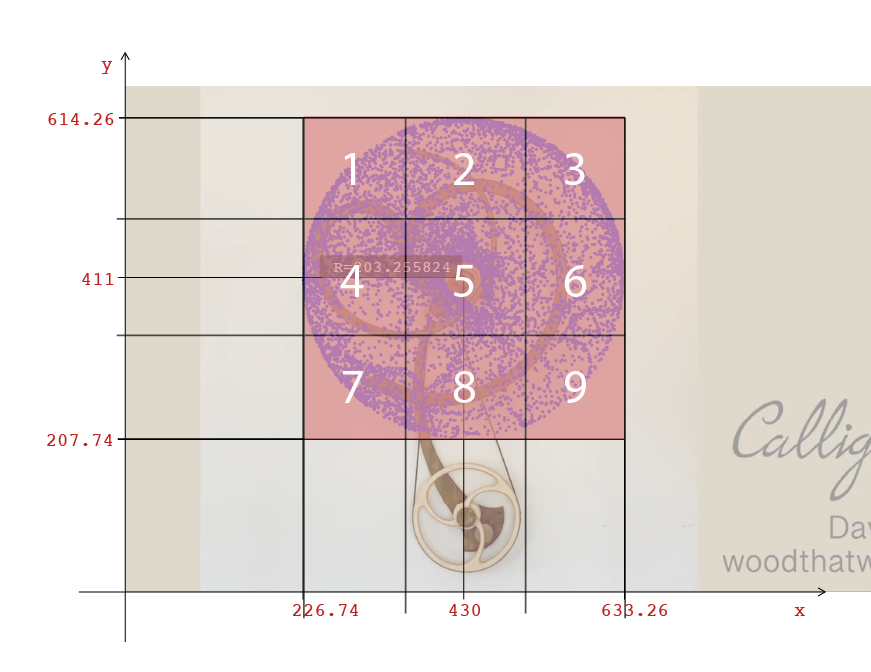
\includegraphics[width=\textwidth]{boxes_sculpt_cartesian} 
        \end{center}
        \caption{}
        \label{fig:boxes_sculpt_cartesian}
    \end{figure}

    Each box has the side of $2R/3 \approx 135.5$.

    Count the number of points in each box. Let $X_i$ be the event of a point being inside box $i$. The results are as following:
\begin{table}[H]
    \centering
    \begin{tabular}{|l|l|l|}
        \toprule
        Box ($i$) & Count & $P(X_i)$\\ 
        \midrule
        1 & 703 & 0.09385847797\\
        2 & 626 & 0.08357810414\\
        3 & 292 & 0.03898531375\\
        4 & 994 & 0.1327102804\\
        5 & 1774 & 0.2368491322\\
        6 & 854 & 0.1140186916\\
        7 & 612 & 0.08170894526\\
        8 & 899 & 0.1200267023\\
        9 & 736 & 0.09826435247\\
        \midrule
        Total & 7490 & 1\\
        \bottomrule
    \end{tabular}  
    \caption{\label{tab:box}Points by box. Software used: MS Excel}
\end{table}   
    Box 5 contains the highest number of points during the period observed, corresponding to a high probability of 23.6\% that the tip of the sculpture ends up inside this area. This figure is up to $\sim$6.2 times the probability of the tip being in box 3. However, the lower probability for boxes number 1, 3, 7, 9 is in a large part due to the grid not perfectly covering the circle-shape collection of points.

    \subsubsection{Group in annuli of equal radii}

    Instead of boxes, the points can also be grouped in annuli of equal radii ($= \frac{R}{3} = 67.7519413$) (Figure \ref{fig:rings_equalRadii})

    \begin{figure}[H]
        \begin{center}
            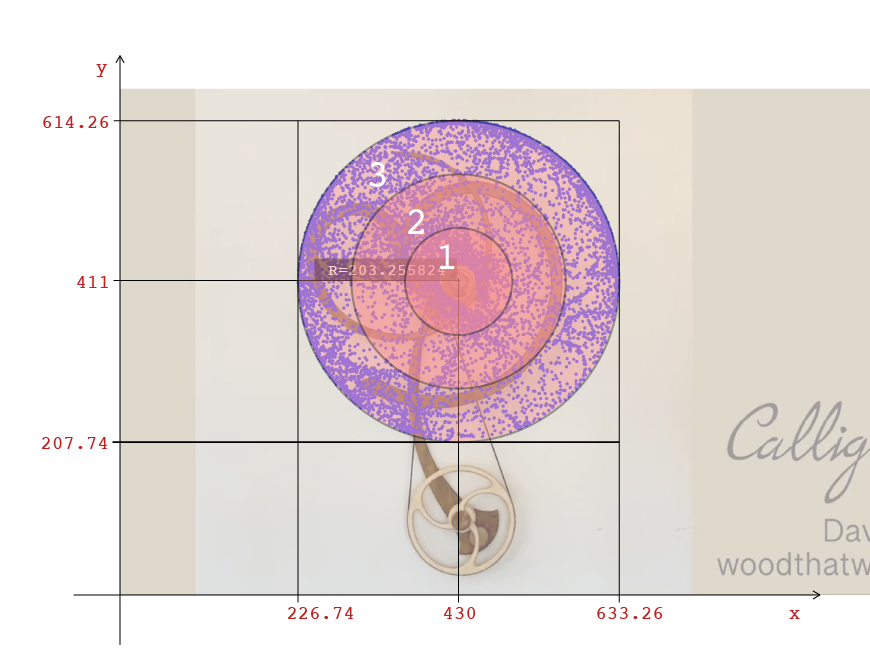
\includegraphics[width=\textwidth]{rings_equalRadii} 
        \end{center}
        \caption{}
        \label{fig:rings_equalRadii}
    \end{figure}
    Let $Y_j$ be the event that a point lies inside annulus $j$. Annuli are labelled in Figure \ref{fig:rings_equalRadii}. Using the software MS Excel to count the number of points inside each annulus, this table is produced:
    \begin{table}[H]
        \centering
        \begin{tabular}{|l|l|l|}
            \toprule
            Annulus ($j$) & Count & $P(Y_j)$\\
            \midrule
            1 & 1579 & 0.2108144192\\
            2 & 1610 & 0.214953271\\
            3 & 4301 & 0.5742323097\\
            \midrule
            Total & 7490 & 1\\
            \bottomrule
        \end{tabular}
        \caption{\label{tab:ring1}Points by annulus, equal radius. Software used: MS Excel}
    \end{table}

    There is a 57.4\% probability that the tip of the sculpture ends up somewhere inside annulus 3 (the outermost annulus) during the period observed. This is much higher than any other annuli: almost three times (2.73 times) the probability for annulus 1 (the innermost annulus), and about 2.6 times the probability of the tip being inside annulus 2 (the middle annulus) .

    However, this can be due to the areas covered by each of the 3 annuli being unequal. Specifically,

    \begin{itemize}
        \item Let area of annulus 1 be $A_1$:
        \begin{center}
            $A_1 = 67.75^2\pi$
        \end{center}
        \item Let the area of annulus 2 be $A_2$:
        \begin{center}
            $A_2=(67.75\cdot2)^2\pi-67.75^2\pi =(2^2-1)67.75^2\pi =3\cdot 67.75^2\pi=3A_1$
        \end{center}
        \item Similarly, let the area of annulus 3 be $A_3$:
        \begin{center}
            $A_3=(67.75\cdot3)^2\pi-(67.75\cdot2)^2\pi =5A_1$
        \end{center}
    \end{itemize}
    %TEACHERCOMMENT: It would be interesting to compare ratio P(Y) / A(Y)
    %The ratio between the number of points being inside an annulus and the area of that annulus can be calculated to mediate this bias. Let $C_i$ be the number of points being inside annulus $i$:
    %\begin{align*}
    %    \frac{C_1}{A_1} &= \frac{1579}{67.75^2\pi} = 0.1094998838 \\
    %    \frac{C_2}{A_2} &= \frac{1610}{3\cdot67.75^2\pi} = 0.03721655328 \\
    %    \frac{C_3}{A_3} &= \frac{4301}{5\cdot67.75^2\pi} = 0.05965281826
    %\end{align*}
    \subsubsection{Group in annuli of equal areas}

    Rather than 3 annuli of equal radii, the data can also be grouped into 3 annuli of equal areas.

    Let the respective outer radius of annulus 1, annulus 2 be $R_1$ and $R_2$; and the area of the big constraining circle covering all the data point be $A$. The outer radius of annulus 3 is obviously also the radius of the big circle ($R$), thus requires no calculation.

    If the 3 annuli are to have equal areas, then:

    \begin{center}
        $A_1=A_2=A_3=\frac{A}{3}=\frac{R^2\pi}{3}$
    \end{center}

    The area of the inner annulus:

    \begin{center}
        $A_1=R_1^2\pi$
    \end{center}

    Rearrange in terms of $R$:

    \begin{center}
        $\frac{R^2\pi}{3}=R_1^2\pi$

        $R_1=\frac{1}{\sqrt{3}}R=\frac{1}{\sqrt{3}}\cdot203.255824=117.3498047$
    \end{center}

    Likewise, for the middle annulus:
    \begin{center}
        \begin{equation}
            \begin{split}
                A_2&=R_2^2\pi-A_1
                \\
                \frac{R^2\pi}{3}&=R_2^2\pi-\frac{R^2\pi}{3}
                \\
                R_2&=\sqrt{\frac{2}{3}}R=165.9576854
            \end{split}
        \end{equation}
    \end{center}

These new values for $R_1$ and $R_2$ are visualized in Figure \ref{fig:ring2} and used to produce Table \ref{tab:ring2}.
\begin{figure}[H]
    \centering
    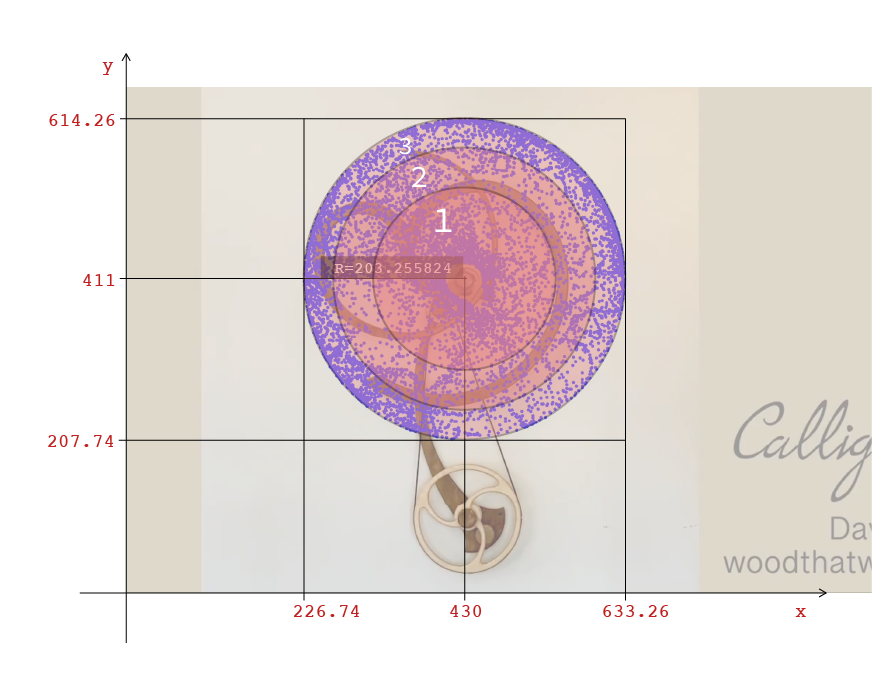
\includegraphics[width=\textwidth]{rings_equalArea}
    \caption{}
    \label{fig:ring2}
\end{figure}
    \begin{table}[H]
        \centering
        \begin{tabular}{|l|l|l|}
            \toprule
            Annulus ($k$)& Count & $P(Y_k)$\\
            \midrule
            1 & 2771 & 0.3699599466\\
            2 & 1441 & 0.1923898531\\
            3 & 3278 & 0.4376502003\\
            \midrule
            Total & 7490 & 1\\
            \bottomrule
        \end{tabular}
        \caption{\label{tab:ring2}Points by annulus, equal area. Software used: MS Excel}
    \end{table}
    Annulus 3 is still where the points are most concentrated, with a 43.7\% chance the tip being in this area during the 250 seconds period recorded. However, annulus 1 now has a significantly higher probability of the tip being there, about 36.98\% compared to only 20.98\% in the previous version where annuli are of unequal areas. It also ranks second now, instead of ranking last among the annuli in terms of the likelihood of being where the tip reached. This corresponds to the visual observation that most points concentrate closer to either the center point or the edge of the circle, but distribute more sparsely in the space in-between (Figure \ref{fig:distribution}).

    \begin{figure}[H]
        \begin{center}
            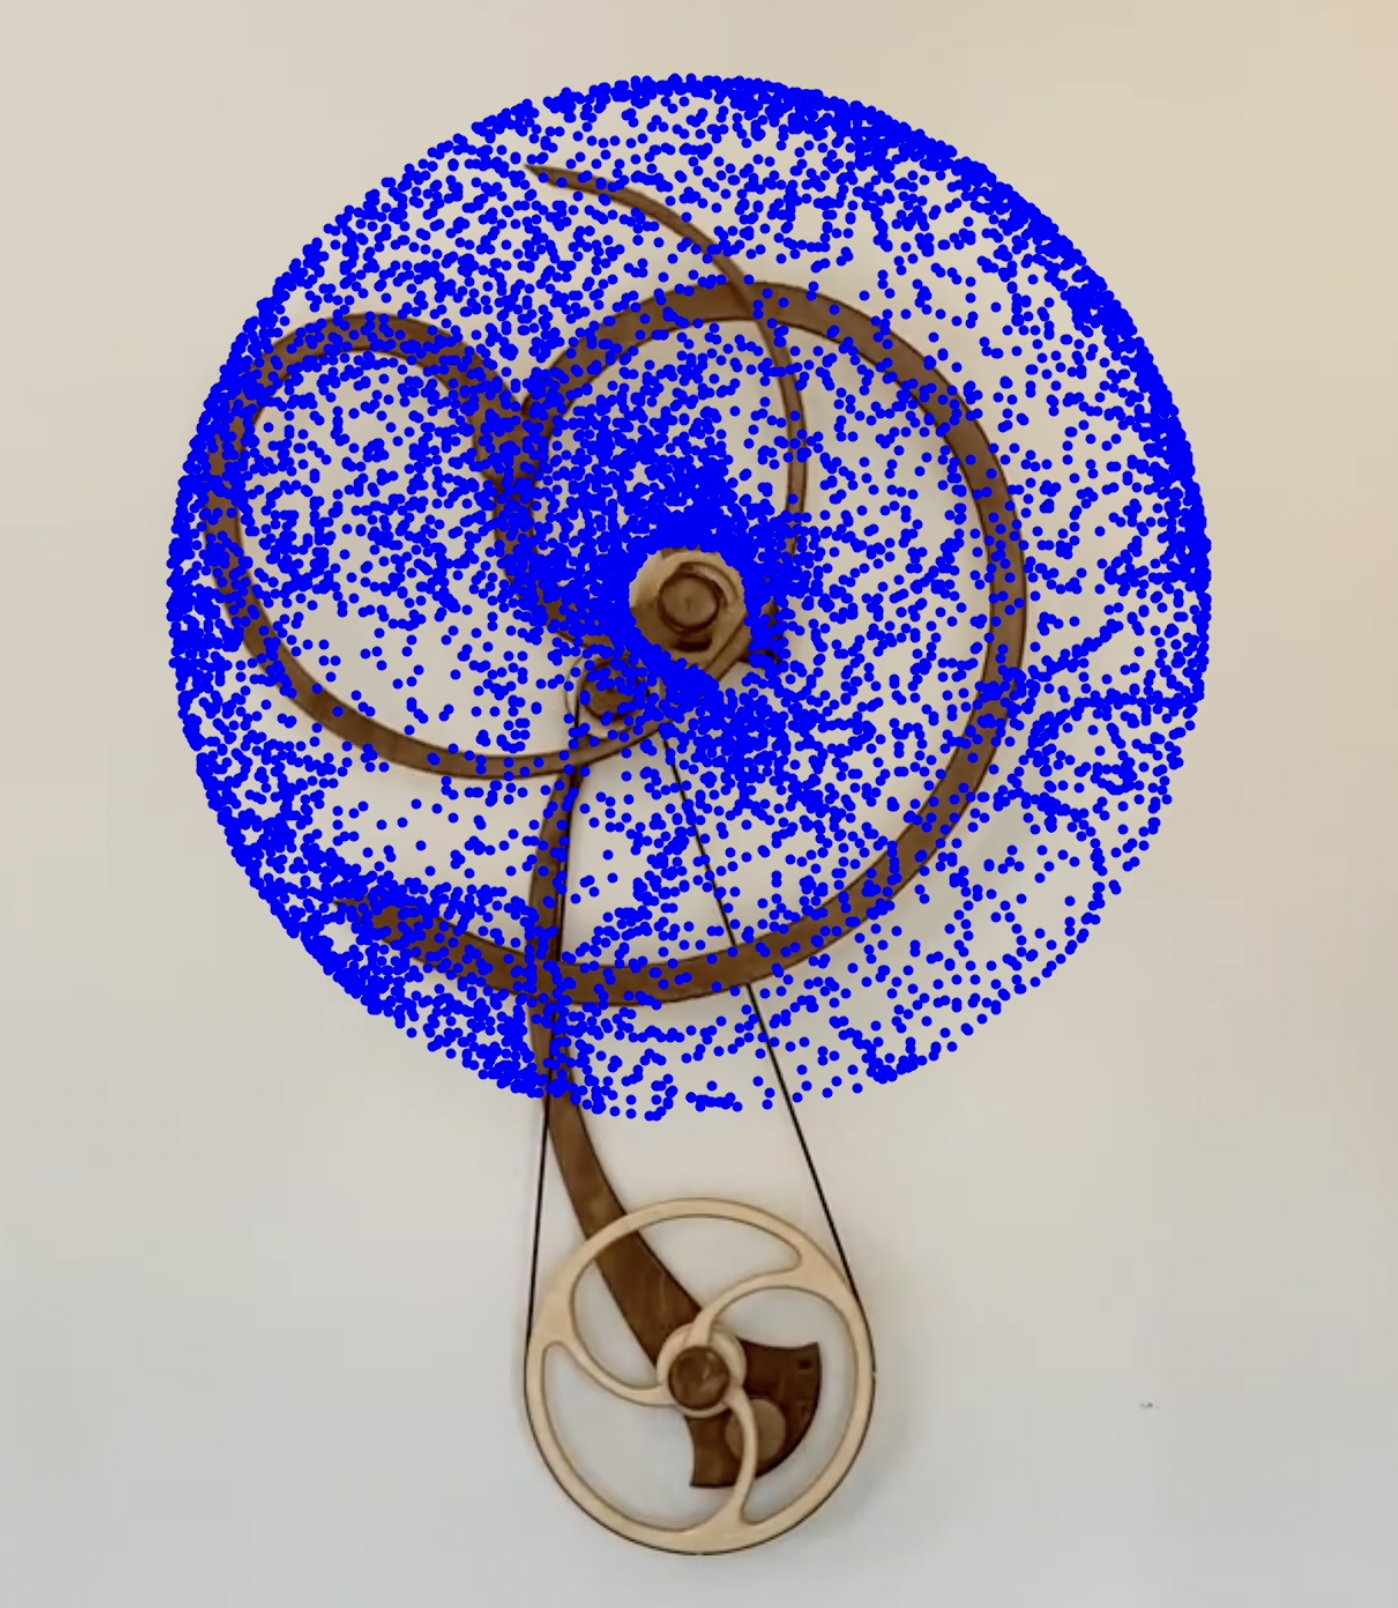
\includegraphics[width=.45\textwidth]{distribution} 
        \end{center}
        \caption{Collection of the points the tip make during the 250-second duration. \\Software used: LoggerPro}
        \label{fig:distribution}
    \end{figure}

    \subsubsection{Probability distribution of distance from tip to pivot point}
    The division by annuli seemed to present the data in a way more meaningful than the division by boxes. Extending on this idea of using the distance from the inner pivot point of the sculpture ($P_1$) to define the tip's position, we can employ the software MS Excel to create a more detailed probability distribution.
    
    Let the distance of a point from $P_1$ $(430, 411)$ be $d_i$. It is given by:

    \begin{equation} \label{eq:14}
        d_i=\sqrt{(x_i-430)^2+(y_i-411)^2}
    \end{equation}

    With $x_i$, $y_i$ being the x and y-coordinates of the point.

    Enter equation (\ref{eq:14}) into the software MS Excel, the software generates a list of distance, $d_1$ to $d_{7490}$. The result can be plotted in a histogram with each interval of width 10:
    \begin{figure}[H]
        \centering
        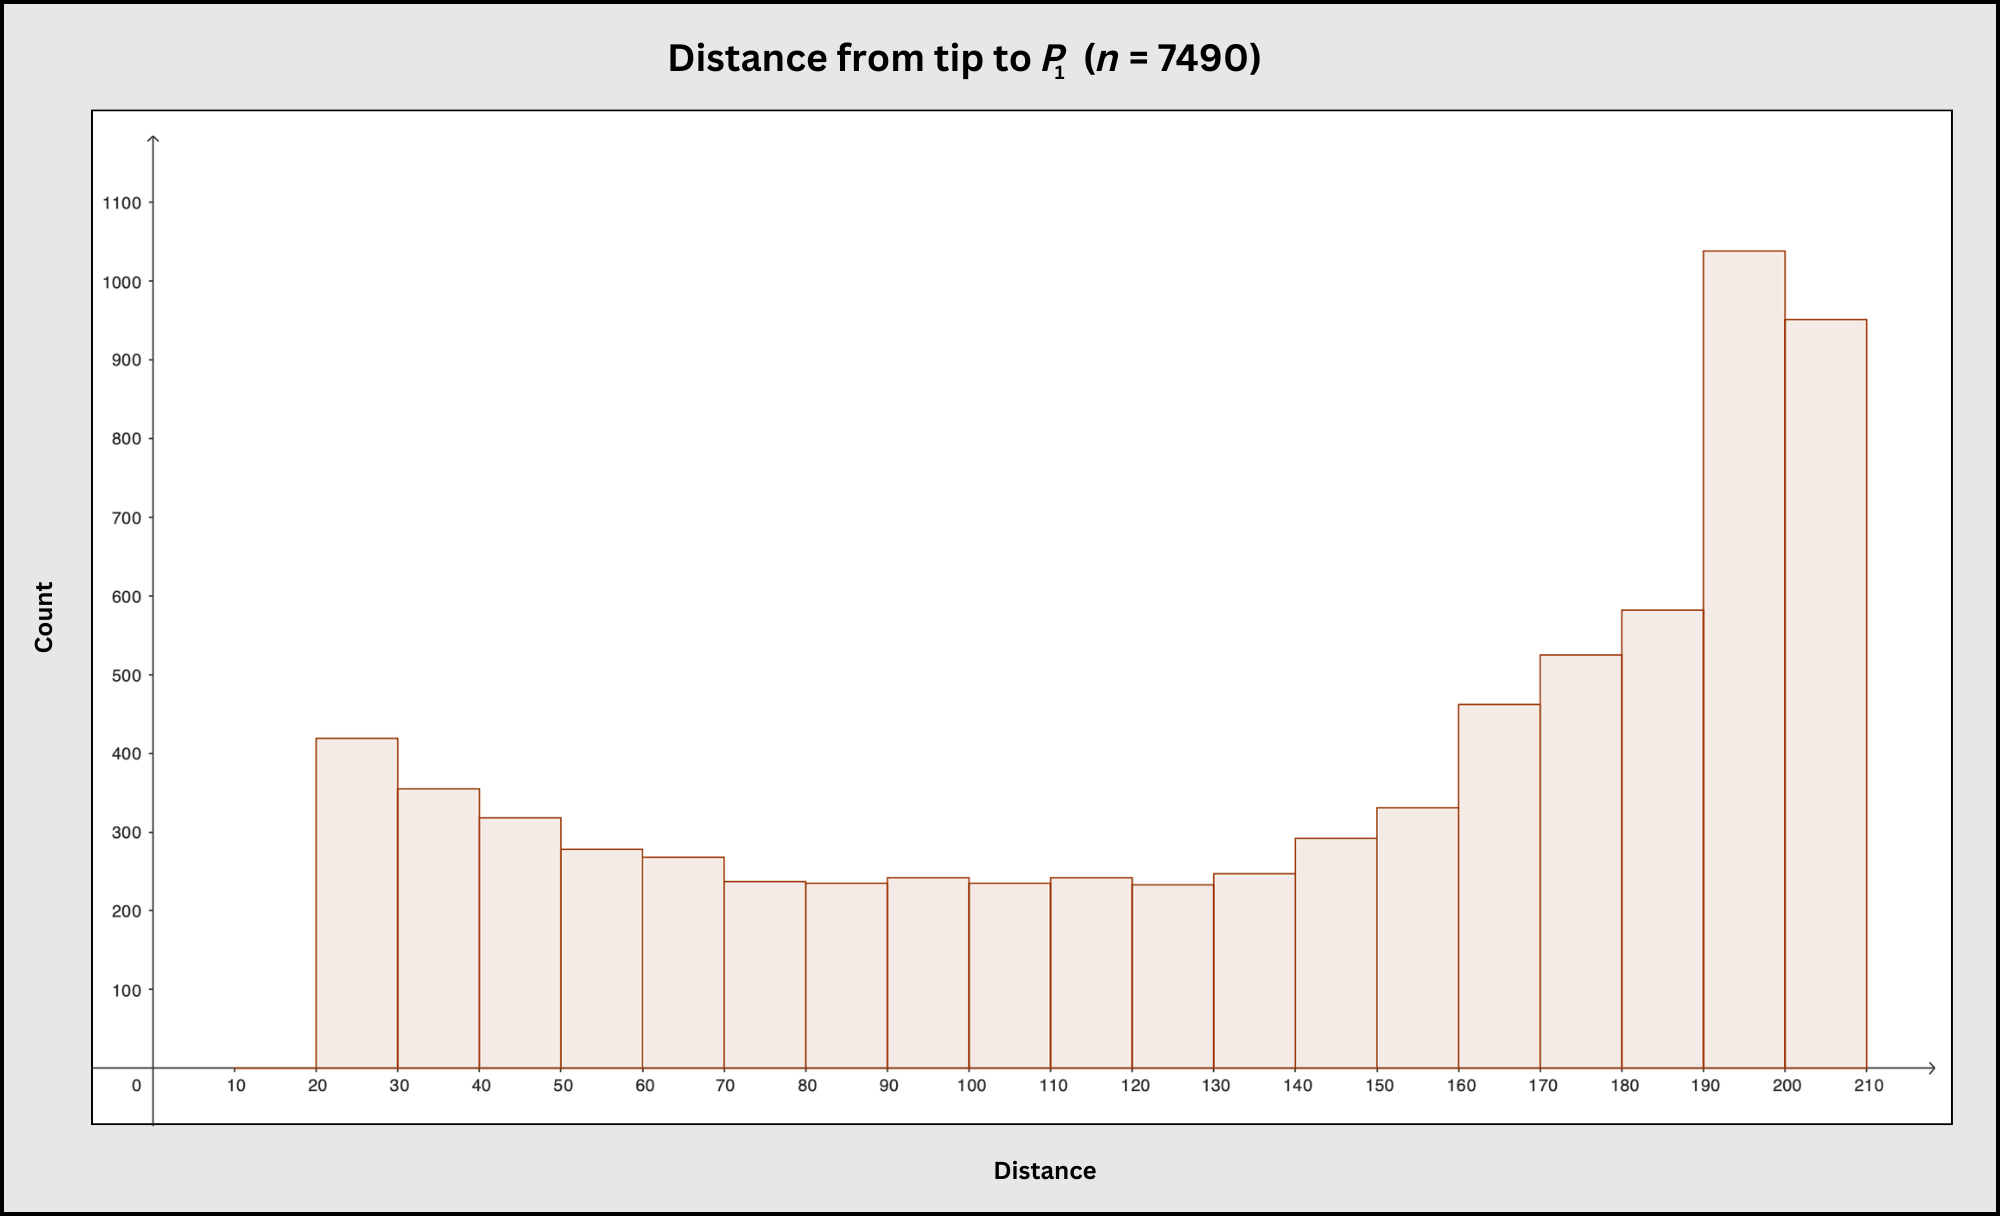
\includegraphics[width=\textwidth]{distance-graph}
        \caption{Histogram of distance from the tip to $P_1$. Software used: MS Excel, Geogebra}
        \label{histogram}
    \end{figure}

    The mean value is calculated using the command AVERAGE(), and the median value using the command MEDIAN() in MS Excel.
\pagebreak

    The software outputs:

    \begin{center}
        $\bar d=135.018458$

        $M=154.4558777$
    \end{center}

    ($\bar d$= mean value; $M$ = median value)

    The range is $d_{max} - d_{min}$ = 204.984226- 21.73432046 = 183.2499055

    It can be observed from both Figure \ref{histogram} and from comparing the mean and median values ($\bar d<M$) that this set of data skews to the left. 
    
    Let $X$ be a discrete random variable. The variance of $X$ is given by:

    \begin{center}
        $Var(X)=E[X^2]-(E[X])^2$
    \end{center}

    Where $E[X]$ and $E[X^2]$ is the expected value of $X$ and $X^2$ respectively \cite{nzmaths}. 

    In our case, $d_i$ is the variable. Since every value of $d_i$ only occur once, the expected value is the mean average:

    \begin{center}
        $E[d_i]=\dfrac{d_1+d_2+...+d_{7490}}{7490}=\bar d$
    \end{center}

    Similarly:

    \begin{center}
        $E[d_i^2]=\dfrac{d_1^2+d_2^2+...+d_{7490}^2}{7490}$
    \end{center}

    Therefore, the variance is calculated to be:

    \begin{center}
        $Var(d_i)=E[d_i^2]-(E[d_i])^2= 21882.12393-135.018458^2=3652.139946$
    \end{center}

    The standard deviation is $\sqrt{3652.139946}=60.43293759$, meaning the distance from the tip of the sculpture to the inner pivot point varies quite a lot, in average being 60.4 ($\approx1/3$ the range) from the mean.

    Figure \ref{histogram} shows a trend in the distribution of the data: the closer to the middle, the less frequent the value. This again corresponds to the visual observation that most points concentrate closer to either the center or the edge, but distribute more sparsely in the space in-between (Figure \ref{fig:distribution}).

    The expected value of $d_i$ is 135.018458, making the expected position of the tip being inside annulus 2 in both senarios where the annuli are of equal radii, or of equal areas. This initially seemed strange, considering the fact that annulus 2 is never the one with the highest probability of the tip being inside it during the 250-second period. In both of the scenarios, annulus 3 has the highest probability of the tip being inside it (57.4\% if equal radii, 43.7\% if equal area). However, this can be explained by the fact that the expected value for the distance is an average of all the distance of the points. From visual observation, most points concentrate either close to the center or on the edge, less often in the area in-between. The average distance of a point close to the center and a point close to the edge would be the measure for the distance of the point between them - likely in the middle annulus, or annulus 2.

    According to information reported by the author of the sculpture \cite{roy-2021}, the real-life width of the sculpture is 40'' = 101.6 cm. The corresponding width in the coordinate system is $2R=2 \cdot 203.255824=406.511648$ (units). Therefore, each cm is equivalent to $406.511648/101.6= 4.00109889764$ units.

    The expected value of $d_i$ is 135.018458. Therefore, the expected value of the real-life distance between the tip and the pivot point of the inner wing is $135.018458/4.00109889764 \approx 33.745$ cm (rounded to the third digit after decimal point)

    %TEACHERCOMMENT: Interesting to see which "ring" this is in? Compare the 2 results.

\subsection{Limitations of the second approach}

Since the data is manually collected by mouse-click points on the video, there is some human error involved. However, the much bigger limitation of this approach is the fact that data are collected for a single trial, with a single set of initial conditions over a limited period of time. Therefore, generalization of the conclusion is subjected to low validity.

\pagebreak
%Conclusion
\section{Conclusion}
This essay is done to answer the research question: \textit{What is the most probable position of David C. Roy’s kinetic sculpture \textit{“Calligraphy”} would a viewer see if they walk in the exhibition during the first 250 seconds after the sculpture starts running?}

For the very specific set of initial conditions in the video examined, the most probable position of the sculpture is one such that the distance from the tip to the pivot point $P_1$ equals 33.745 cm.

However, according to the analysis of the simple double pendulum, and assuming damping and forcing do not eradicate the chaotic nature of the system, the behavior of \textit{“Calligraphy”} is highly sensitive to initial conditions. Meanwhile, in reality, there will be a certain margin of error when measuring the dimensions or setting the sculpture to a specific state. This means it would be impossible to predict the trajectory of the sculpture in real life, since that small margin of error in initial conditions can magnify into large difference in the predicted versus the actual trajectory. 

Further research is needed to understand the behavior of \textit{“Calligraphy”}. With the first approach, the area of improvement is to include the effects of the changed centre of mass, added energy from the spring, and damping from friction and air resistance. With the second approach, data of a larger number of trials with a controlled set of initial conditions is needed to produce results of statistical significant.
\pagebreak
%Bibliography
\printbibliography
\clearpage
\pagenumbering{roman}
%Appendices
\begin{appendices}
    \section{Source code}
        MATLAB code to solve and graph results of equations $(12)$ and $(13)$.
        \begin{verbatim}
% declare symbolic variables.
syms theta_1(t) theta_2(t) L_1 L_2 m_1 m_2 g;

% declare the equations of motion.
% (rearranged for cleaner code)
w_1 = diff(theta_1);
w_2 = diff(theta_2);
alpha_1 = (L_2/L_1)*(m_2/(m_1 + m_2))*cos(theta_1 - theta_2);
alpha_2 = (L_1/L_2)*cos(theta_1-theta_2);
f_1 = -(L_2/L_1)*(m_2/(m_1 + m_2))*diff(theta_2)^2*sin(theta_1-theta_2)
-(g/L_1)*sin(theta_1);
f_2 = (L_1/L_2)*diff(theta_1)^2*sin(theta_1-theta_2)-(g/L_2)*sin(theta_2);

% actual equations of motion,
% built from previously declared equations.
symsEqn_1 = diff(w_1) + alpha_1*diff(w_2) == f_1;
symsEqn_2 = diff(w_2) + alpha_2*diff(w_1) == f_2;

% substitute symbolic variables with real values.
eqn_1 = subs(symsEqn_1,[L_1 L_2 m_1 m_2 g],[1 1 1 1 9.8]);
eqn_2 = subs(symsEqn_2,[L_1 L_2 m_1 m_2 g],[1 1 1 1 9.8]);

% reduce to first-order differential equations,
% returned as a symbolic vector.
[V,S] = odeToVectorField(eqn_1,eqn_2);

% convert to MATLAB function
M = matlabFunction(V,'vars',{'t','Y'});

% replace theta1 and theta2 with real values.
% WARNING: Code won't work unless real values
% are substituted in.
% eg: initCond = [0 0 pi/12 0];
initCond = [theta2 0 theta1 0];

% solves the differential equation, t spanning
% from 0 to 20.
sols = ode113(M,[0 20],initCond);

% extracting theta1 (column 3) and theta2 (column 1)
% from the solution, to plot only theta1 and theta2
solstheta = sols.y([3 1],:);

% plotting the solution
plot(sols.x,solstheta)
legend('\theta_1','\theta_2')
title('Solutions of State Variables')
xlabel('Time (s)')
ylabel('Solutions (rad)')
        \end{verbatim}
    \section{Raw data}
        List of data about tip position of the sculpture “Calligraphy” during the 250-second period.

        Since the table is too long (3 columns, 7591 rows) to be attached to this document, a .csv file has been generated and made downloadable through the following link:

        \url{https://docs.google.com/spreadsheets/d/1BdqeAavf2CFdXiNE7JpukFZzKib1UwZ4f1KGYdxuU8w/gviz/tq?tqx=out:csv}
\end{appendices}
\end{document}